\documentclass[11pt,usenames,dvipsnames,svgnames,x11names]{beamer} 

\usetheme{Warsaw}
\usepackage{amssymb,amsmath,amsthm,amsfonts}                    
\usecolortheme{whale} 
\setbeamertemplate{navigation symbols}{}
\usepackage[utf8]{inputenc} 
\usepackage{polski}
\usepackage{tikz}
\usepackage{subfigure}
\usepackage{setspace}
\usepackage{savesym}
\savesymbol{arc}
\usepackage{color}
\usepackage{xcolor}
\usepackage{pict2e}
\usepackage{epstopdf}
\usepackage{caption}
\usepackage{graphicx}
\usepackage{pict2e}
\usepackage{epstopdf}
\usepackage{geometry}
\usepackage{mathabx}

\date{2 czerwca 2014}
\author{Kamila Komar i Marta Sommer}
\title{ANOM - analiza średnich}

\theoremstyle{plain}
\newtheorem{twierdzenie}{Twierdzenie} 
\newtheorem{twierdzeniecd}{Twierdzenie cd.} 
\theoremstyle{definition}
\newtheorem{definicja}{Definicja}
\newtheorem{przyklad}{Przykład}
\newtheorem{lemat}{Lemat}
\newtheorem{wniosek}{Wniosek}
\newtheorem{oznaczenia}{Oznaczenia}
\theoremstyle{remark}
\newtheorem{uwaga}{Uwaga}

\begin{document}


\begin{frame}   
\titlepage
\end{frame}

%%%%%%%%%%%%%%%%%%%%%%%%%%%%%%%%%%%%%%%%%%%%%%%%%%%%%%%%%%%%%%%%%%%%%%%%%%%%%%%%%%%%%%%%%%%%%%%%%%%%%%%%%%%%%%%%%%%%%

\begin{frame}
\frametitle{Po co nam ANOM?}
Jednoczynnikowa ANOM - mamy $k$-poziomów jednego czynnika. Sprawdzamy, czy średnia w jednym z poziomów różni się istotnie od średniej ze wszystkich poziomów. ANOVA badała, czy średnia różni się od którejś ze średnich innych czynników. ANOM bada, czy średnia różni się od średniej ze wszytkich czynników.  
\end{frame}


\begin{frame}
\frametitle{Porównanie metod}
%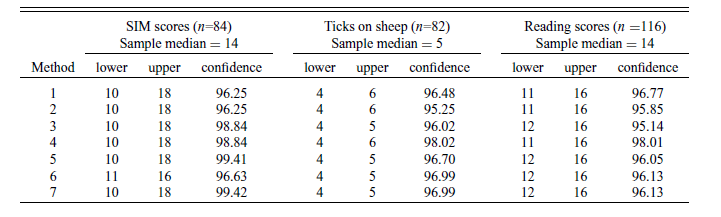
\includegraphics[width=\textwidth]{5.png}
\end{frame}

\begin{frame}
\frametitle{Bibliografia}
\begin{thebibliography}{9}
\bibitem{budyn1} Thomas P. Ryan, Statistical~Methods~for~Quality~Improvement, WILEY (1989), rozdział 16.
\end{thebibliography}
\end{frame}


\end{document}
